1. Common problems and common technologies [+]
 - Text search +
 - Self Index +
 - Problems with self indexation +
 - Full text search with substrings +
2. SA: overview, complexity, usage         [+]
3. Radix: overview, complexity, usage      [+]
4. Succinct data                           []
5. CSA                                     []
6. PSI                                     []
7. EF                                      []
6. My CSA                                  []
8. Complexity

\textbf{Поиск по тексту}

В настоящее время Интернет каждый день пополняется большим количеством данных.
Поэтому чрезвычайно важно организовать поиск нужной информации \emph{эффективно}.
При поиске по документам применяется индексирование.
Традиционным для индексирования текста является \emph{inverted index}.
Это структура данных, в которой для каждого слова коллекции документов в соответствующем списке
перечислены все документы в коллекции, в которых оно встретилось.
При обработке многословного запроса берётся пересечение списков, соответствующих каждому из слов запроса.

\textbf{Проблемы традиционных подходов}

На практике встречаются случаи, в которых невозможно использовать традиционный поиск по словам.
Модель поиска, в которой задачей является найти орфографически близкие слова (\emph{fuzzy search}),
использующаяся для корректирования правописания во многих текстовых редакторах,
не позволяет решать проблему при помощи поиска по словам.
То же самое касается других систем, в которых используется \emph{pattern matching}.
Еще одним примером текстов, в которых невозможно применять традиционный поиск,
являются некоторые восточные языки.
В них слова не делятся пробелами между собой, что делает трудным использование \emph{inverted index}.
Наконец, к "неудобным" можно отнести длинные тексты, составленные из алфавита с малым набором символов.
Характерными примерами таких текстов являются ДНК и код белковой структуры.
Этот текст к тому же тоже не делится на слова.

Во всем вышеприведенных случаях текст не делится на слова,
поэтому для таких примеров необходимо использовать поиск по подстрокам.
Существующие подходы (prefix tree, suffix array) занимают много места, поэтому не являются эффективными.
Например, для prefix tree, хранящем в себе n слов со средним количеством символов в каждом слове C,
требуется $O(n \cdot C)$ памяти.
Рассмотрим подробнее suffix array, как один из самых востребованных способов индексации текстовой информации.

\textbf{Полнотекстовый поиск при помощи suffix array}

Suffix array -- это структура данных, используемая в полнотекстовой индексации, позволяющая выполнять
поиск подстроки в тексте размером n символов за $O(\log{}n)$.
При этом для хранения n слов в suffix array необходимо $O(n \log{}n)$ памяти.
Так для ASCII-текста размером $2^{32}$ требуется $2^{32} \cdot 8 = 32$ гигабит пространства памяти.
Для такого текста suffix array должен содержать элементы размером 32 бита.
Тогда размер suffix array достигает $2^{32} \cdot 32 = 128$ гигабит пространства памяти,
что в 4 раза превышает размер исходного текста.

\textbf{Создание suffix array}

Suffix array представляет собой отсортированную в лексикографическом порядке
последовательность суффиксов. Для лучшего понимания устройства suffix array, рассмотрим эту структуру данных на примере индексирования
слова mississippi:
\\(0) mississippi
\\(1) ississippi
\\(2) ssissippi
\\(3) sissippi
\\(4) issippi
\\(5) ssippi
\\(6) sippi
\\(7) ippi
\\(8) ppi
\\(9) pi
\\(10) p

Suffix array, составленный из таких суффиксов, будет иметь вид:

7 4 1 0 10 9 8 6 3 5 2

Обычно конец документа обозначается специальным символом, не входящим в алфавит хранящегося в массиве текста.
В качестве такого разделителя в этой работе был выбран символ доллара \$.
Современные подходы по построению suffix array позволяют конструировать структуру данных за $O(n)$.

\textbf{Radix tree}

% Picture By Claudio Rocchini - Own work, CC BY 2.5, https://commons.wikimedia.org/w/index.php?curid=2118795

\begin{wrapfigure}{r}{0.25\textwidth} %this figure will be at the right
 \centering
 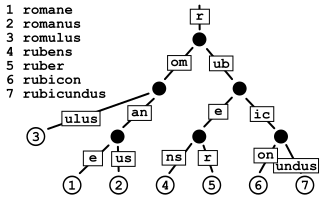
\includegraphics[width=0.45\textwidth]{PatriciaTrie}
\end{wrapfigure}

Radix tree представляет собой сжатое prefix tree. В свою очередь, prefix tree является
структурой данных, которая предоставляет интерфейс ассоциативного массива и позволяет
хранить значения в виде key-value пар.
В этом исследовании в качестве key выбраны строки, причем в отличие от обычный деревьев,
на ребрах radix tree могут храниться как один элемент (символ),
так и последовательность элементов (строка).

Radix tree широко применяется в ядре Linux для связи указателя с длинным целочисленным ключом.
Эта структура данных эффективна с точки зрения скорости поиска и хренения информации.
В то же время, Radix tree применяется в IP-адресации, так как очень удобна для хранения
иерархической структуры IP-адресов.

\textbf{Поиск и хранение данных в radix tree}

Рассмотрим подробнее характеристики radix tree. Пусть требуется хранить ключи размером k
при хранении n элементов в дереве. Тогда добавление элемента, поиск и удаление элемента
занимают $O(k)$ операций.

Для многих запросов поиска по словарю radix tree может быть быстрее и эффективнее, чем хеш-таблицы.
Несмотря на то, что обычно сложность поиска по хэш таблице принимают за $O(1)$,
при этом игнорируется необходимость сначала хешировать входные данные.
На это обычно требуется $O(k)$ операций, где k -- длина входной строки.
Radix tree выполняет поиск за $O(k)$, без необходимости сначала хешировать и имеют гораздо лучшую локальность кеша.
Они также сохраняют порядок, позволяя выполнять упорядоченное сканирование,
получать минимальные / максимальные значения, сканировать по общему префиксу и т.д.

Благодаря всем этим преимуществам, radix tree широко распространено в базе данных Redis, программных продуктах
компании HashiCorp, таких как Terraform, Consul, Vault, Nomad и т.д.,
что представляет дополнительный интерес для его изучения на текстовых данных и сравнения с suffix array.

\textbf{Сжатое представление данных}

Одной из главных задач этой работы является разработка сжатого хранения индекса для suffix array.
Поэтому важно определить, какие данные можно считать сжатыми.

Существуют различные степени сжатости информации.
Предположим, что для хранения некоторого количества данных требуется Z бит.
Сжатые (succinct) структуры данных занимают \(Z + o(Z)\) бит, implicit -- \(Z + o(1)\) бит и
compact -- \(O(Z)\)) бит. В этой работе предлагается сжать suffix array, представив его в succinct виде.
Таким образом, размер массива немногих больше превосходит размер исходного текста.


